\documentclass{exam} 
\usepackage{amsmath,amssymb,enumitem,fdsymbol,float,tikz,etoolbox,ifthen,xcolor,fullpage,ulem,graphicx, comment,hyperref,tikz,mhchem} 
\graphicspath{{./Images/}}
\setlength\parindent{0in}
%\pagestyle{empty}

\everymath{\displaystyle}
\newcommand{\dee}{\,\text{d}}
\newcommand{\diff}[2]{\frac{\text{d}#1}{\text{d}#2}}

\begin{document}

\large{\textbf{ASSIGNMENT 1}}

\normalsize




\subsubsection*{Contributors}

% Students: edit in your names here or these people will get credit for your work 

\begin{itemize}
    \item \#66220104 David {\bf Jiang} 
    \item \#71389423 Adam {\bf Long}
    \item \#42692376 Zhuyue {\bf Wu}
\end{itemize}

\

\hrulefill

\

\textbf{Reflection question}

\

\textit{Reflection questions encourage you to think about how mathematics is done. This is an important ingredient of success. Reflection questions contribute to your \textbf{engagement grade}.}

\begin{questions}

\question To work productively as a team, it is helpful to have shared expectations. This question consists of prompts that form a ``team contract'', a document that guides how you will work together. Before answering the prompts, read the document ``Group resources'' that is posted along with the assignment on the Canvas course page.

\begin{parts}
    \part What are your overarching ``ground rules''? Come up with 4-6 specific expectations regarding communication (including how often and what medium), meetings (how often, how long, and where), preparation and attendance.
    \part What actions will your team take if a member does not follow the ground rules? Be specific.
    \part What happens if a team member does not fulfill an agreed-upon task for an assignment? Consider both how the team will handle any dropped tasks, as well as  actions you will take as a team.

\end{parts}

\color{blue}
\subsubsection*{Answers}
\begin{parts}
    \part
    The expectations for each member of the group are as follows:
    \begin{enumerate}
    \item Members are expected to inform groupmates should they be unable to complete an assigned question.

	\item Members are expected to work through questions assigned to them to the best of their ability. They are also expected to ask for help should they get stuck on a question.

	\item Members are expected to attend all scheduled meetings absent extraneous circumstances. If a member is unable to attend a meeting, they are expected to notify groupmates beforehand.

	\item Members are expected to provide a reasonable means through which they can be contacted and have a responsibility to acknowledge communications in a timely manner. Failure to acknowledge communications via a means which the group member has deemed reasonable is not an acceptable excuse for missing scheduled meetings or failing to complete assigned groupwork.
	\end{enumerate}

    \part
    If a member fails to follow ground rules or engages with them in bad faith, they may be subject to the following repercussions:
	\begin{itemize}
	\part The first time a member violates an expectation stated above, insofar that they have attempted to adhere to the rules in good faith, they will receive a warning.
	\part The second time a member violates an expectation stated above, their misconduct will be listed in the assignment, though they will not be marked as "non-contributing."
	\part All further violations of the expectations stated above will result in being labelled as "non-contributing" on the assignment during which the violation has taken place.
	\part If a member violates the expectations stated above and groupmates deem that the individual is not attempting to adhere to the ground rules in good faith, there will be no warning and the member will be listed as "non-contributing."
	\end{itemize}
	
	
    \part The actions the group will take in response to a member failing to complete an assigned task are as follows:
    \begin{itemize}
     \part If a group member fails to complete an assigned task but demonstrated reasonable attempts to do so, they will be assisted by groupmates in both understanding the material and completing the task, although they will be expected to notify the group should they be unable to complete a task in the future.
    
    \part If a group member has not started their assigned task but has a valid reason for being unable to do so, the task will be assigned to other group members and the group member in question will be assigned another task.
    
    \part If a group member does not complete an assigned task and provides no valid reason for failing to do so, the consequences will be the same as if they had violated a ground rule. 

    \end{itemize}
\end{parts}
   
\color{black}

\end{questions}



\hrulefill

\

\textbf{Assignment questions}

\

\textit{The questions in this section contribute to your \textbf{assignment grade}. Starred questions are at the level of Part 2 exam questions.}

\begin{questions}\setcounter{question}{1} 

\question\label{original} ($\bigstar\bigstar\largewhitestar\largewhitestar$)

We are going to consider the classical gravitational force associated with the planet Earth. Forces are vector quantities, which have magnitudes and directions, but we will focus on the scalar functions associated with these forces. 

Let's assume Earth is a perfect sphere. Let's also assume the material making up Earth is uniformly distributed throughout this sphere, meaning the density of the Earth is uniform. (This is not true in reality as the core of the Earth is denser than the crust, for example.) 

Suppose Earth has a radius $r_E$ and that we measure distances $r$ to any object from the centre of Earth, which we say is $r=0$. Since we are interested in understanding the gravitational force of Earth alone, it is useful to imagine this object to be small and to have small mass since we will ignore the gravitational force produced by this object itself.

Physics tells us the gravitational force due to the mass of Earth on our small object will only depend on the distance $r$ this object is from the centre of Earth.  We would like to find a function $F$ to describe the gravitational force as a function of the distance $r$. 

For distances $r$ that are greater than $r=r_E$, Newton's law tell us the gravitational force of Earth on our small object is proportional to the inverse of the squared distance $r$; that is, $F(r)=\alpha/r^2$.

If we imagine drilling a hole from the surface of Earth to its centre and placing our object at some depth in this hole a distance $r$ from the centre, then an interesting application of Gauss's law tells us the gravitational force on our small object is proportional to its distance $r$ from the centre of Earth; that is, $F(r)=\beta r$.

\begin{enumerate}

\item[(a)] Find the explicit expression of the function $F(r)$ that describes the gravitational force associated with Earth, where $r\geq 0$. 


\item[(b)] Sketch a graph of $F(r)$ and write a few observations about this function and its graph. What do you know about the gravitational force at the surface of Earth and what does this tell you about the function $F(r)$ when $r=r_E$? What do you know about the relationship between the constants of proportionality $\alpha$ and $\beta$?

\end{enumerate}

\textit{Hint:}  The function  $F(r)$ will be a piecewise defined function; it has a different form for distances that place the object inside Earth than for objects outside Earth's surface. 

\color{blue}
\subsubsection*{Answers}
\begin{parts}
    \part
    	\begin{equation}
    	F(r) = \begin{cases}
    	\frac{\alpha}{r^2} \quad &\text{if} \, r > r_E \\
    \beta r \quad &\text{if} \, 0 \le r < r_E
    	\end{cases}
    	\end{equation}
    \part The following is a graph of force as distance of the object from Earth changes.
    
    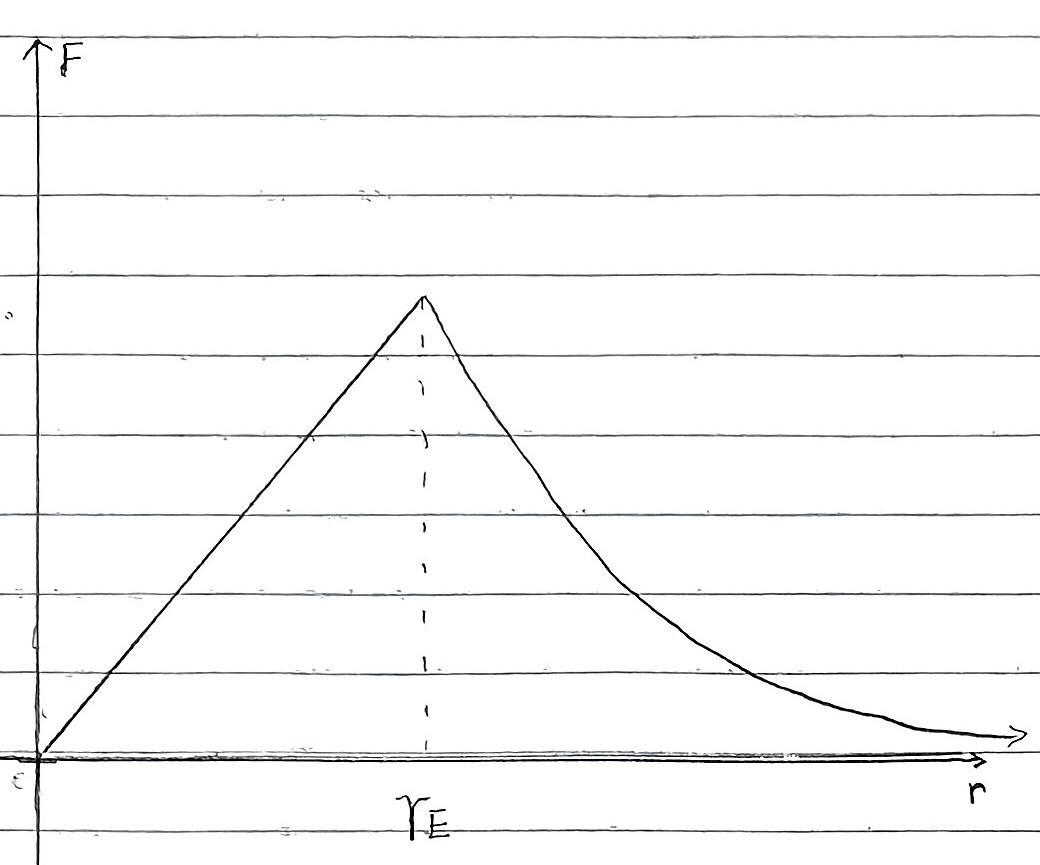
\includegraphics[scale=0.25]{question2graph}
    
    We know experimentally that the acceleration of objects at the Earth's surface is $9.81 m/s^2$. In the graph above, the distance from the center of the Earth to its surface is labelled $r_E$. We can therefore conclude that the force $F$ at $r = r_E$ is $9.81 m/s^2$ multiplied by the mass of the object. Since $F(r)$ is continuous in the interval $[0, \infty)$, we know that $\frac{\alpha}{r^2} = \beta r$ where $r = r_E$. We can therefore find the proportionality of $\alpha$ and $\beta$ using the equation:
    \begin{align*}
    \frac{\alpha}{r_E^2} &= \beta r_E \\
    \alpha &= \beta r_E^3
    \end{align*}
\end{parts}
\color{black}


\question\label{p} ($\bigstar \bigstar \bigstar \largewhitestar$)

Let us consider now a slightly more realistic model of the internal structure of Earth. In particular, imagine the material inside Earth is still distributed with spherical symmetry, meaning the density only depends on the distance from the centre of Earth, but the density of the material varies with this distance. Suppose there is a dense central core of radius equal to $0.4r_E$ of uniform (constant) high density, where $r_E$ is the radius of Earth. This core is surrounded by a mantle of uniform (constant) density that is 60\% of the density of the core.

Let's find the gravitational force on a small object placed at a point inside this Earth. 

Since we are only looking inside the planet, we will measure distances from the centre of Earth as a fraction of Earth's radius. Call this fractional distance $R$ and so $R$ goes from 0 (the centre of Earth) to 1 (the surface of Earth). In terms of the usual distance $r$, we have $R=r/r_E$.

The gravitational force on a small object in the core is $F_c(r)= 1.6r$. 

The expression for the gravitational force on a small object in the mantle is slightly more complicated: $F_m(r)= \frac{0.04}{r^2}+r$.
\begin{enumerate}
\item[(a)] Write down the function $F(r)$ describing the gravitational force an object will experience anywhere inside Earth given this model of Earth's internal structure.

\item[(b)] Sketch a graph of this function.

\item[(c)] If you drilled a narrow hole from the surface straight to the centre of Earth and dropped a small object into this hole, describe carefully how the object would accelerate as it fell towards the centre. (Remember Newton's Second Law says $F=ma$.)

\item[(d)] Some approximations were made to produce the numerical constants in the expressions for the gravitational forces in the core and in the mantle. How can you tell these constants are not given exactly based on properties of the function $F(r)$?

\end{enumerate}

\color{blue}
\subsubsection*{Answers}
\begin{parts}
    \part1
    \begin{equation}
    F(R) = \begin{cases}
    1.6 R \quad &\text{if} \, 0 < R \le 0.4 \\
    	\frac{0.04}{R^2}+R \quad &\text{if} \, 0.4 < R < 1
    
    \end{cases}
    \end{equation}
    \part The following graph depicts the gravitational force exerted on an object inside of Earth's surface:
    
    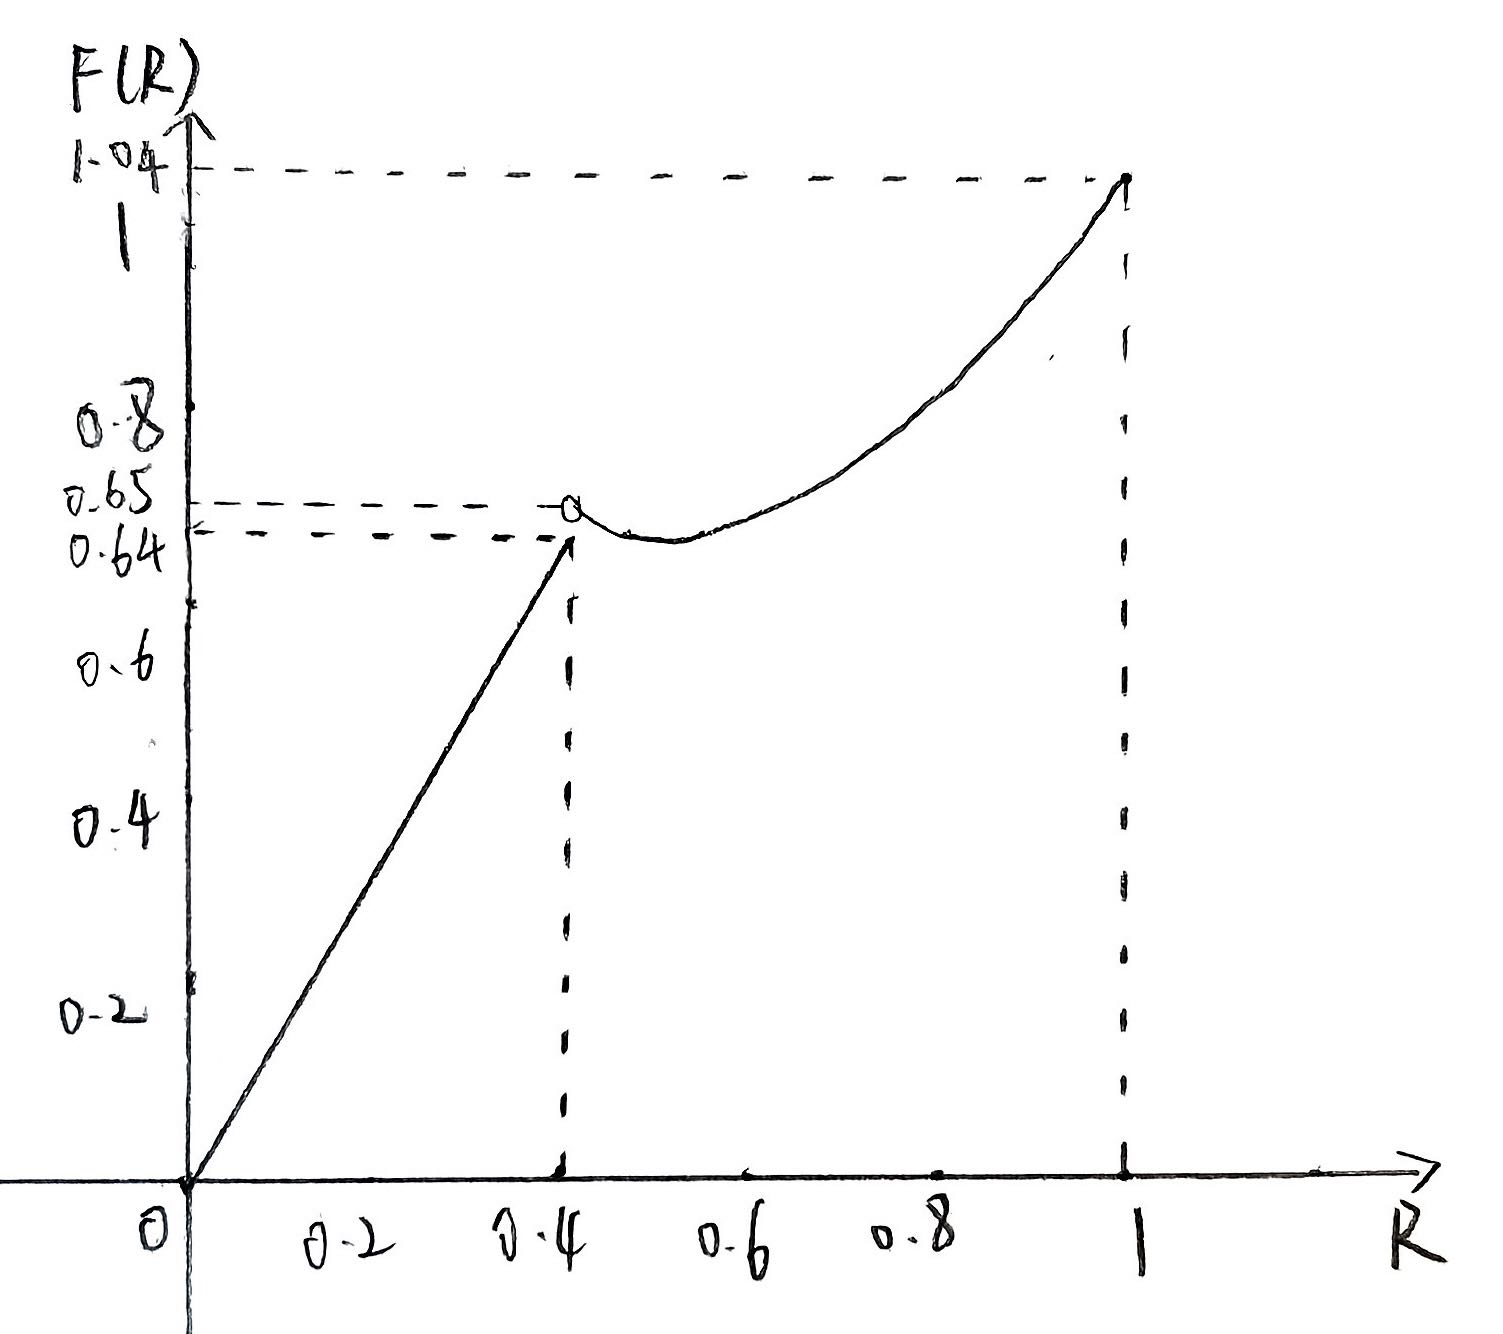
\includegraphics[scale=0.25]{question3graph}
    \part Assuming that air resistance is negligible, the ball would initially accelerate at the highest acceleration it will experience throughout the fall (we experimentally know this to be at $9.81m/s^2$). As the ball falls though the mantle, its acceleration will gradually decrease in a manner that appears linear. However, as the ball nears the inner end of the mantle and beginning of the core, the ball's acceleration will once again increase briefly at an exponential rate. When the ball leaves the mantle and enters the core, its acceleration will begin to decrease again at a linear rate, with the acceleration approaching 0 as its fractional distance to the Earth's core approaches 0.
    \part We can tell that the values given in this question are approximated because, when the gravitational force as a function of R is graphed, there is a jump discontinuity where the mantle and core connect at $R=0.4$. Physically, we know this to be impossible because an instantenous change in acceleration (wherein $\delta t \rightarrow 0$) would require an infinite amount of jerk, which is both theoretically impossible and has never been recorded when an object in real life passes the mantle into the core. Due to this, we know that the actual graph of the acceleration of an object from the Earth's surface to its center would be continuous at the interval $(0,1)$, meaning that the coefficients of R in this case must have been approximated to produce this discrepancy.
\end{parts}
\color{black}

\question ($\bigstar \bigstar \bigstar \largewhitestar$) 

In 1970, science fiction author Larry Niven wrote \textit{Ringworld}, in which there is a large artificial world constructed as a ring that has a diameter approximately the same size as Earth's orbit around the Sun, which means the circumference of Ringworld is about 1 billion kilometers. The total mass of this world is about $2 \times 10^{27}$ kilograms (about 333 times the mass of Earth), which means it has a large gravitational field. For the purposes of this question, we will consider this mass to be uniformly distributed around the ring.

While it is tricky to calculate exactly this gravitational field at a general point in space around this world, the symmetry of Ringworld about an axis running through the centre of the ring and perpendicular to the plane of the ring makes it possible to calculate exactly the gravitational force a small object placed anywhere on this axis will experience. 

The easiest place to calculate the gravitational force is at the centre of the ring:  it must be exactly 0 there because of the symmetry since each bit of the ring has a corresponding bit of the ring of equal mass diametrically opposite to it on the ring. These antipodal bits of the ring exert equal and opposite gravitational forces on a small object at the centre, meaning the net force there is 0 (technically, the gravitational force is a vector, so this is the 0-vector, but we will focus on the magnitude of it, which is the scalar 0). This is true for all such bits of the ring and so their total contributions add up to 0 at the centre of the ring. 

Now consider the axis that passes through the centre of the ring, and that is perpendicular to the plane of the ring. Think of this axis as a straight line acting as a coordinate line where the origin of the coordinate is at the centre of the ring. Let's call this coordinate $z$ and say $z=0$ is the centre. If $z>0$, then we are looking at points in one direction along this axis, and when $z<0$, we are considering points in the other direction. (The choice of positive direction is arbitrary.) 


\begin{figure}[h]
\begin{center}
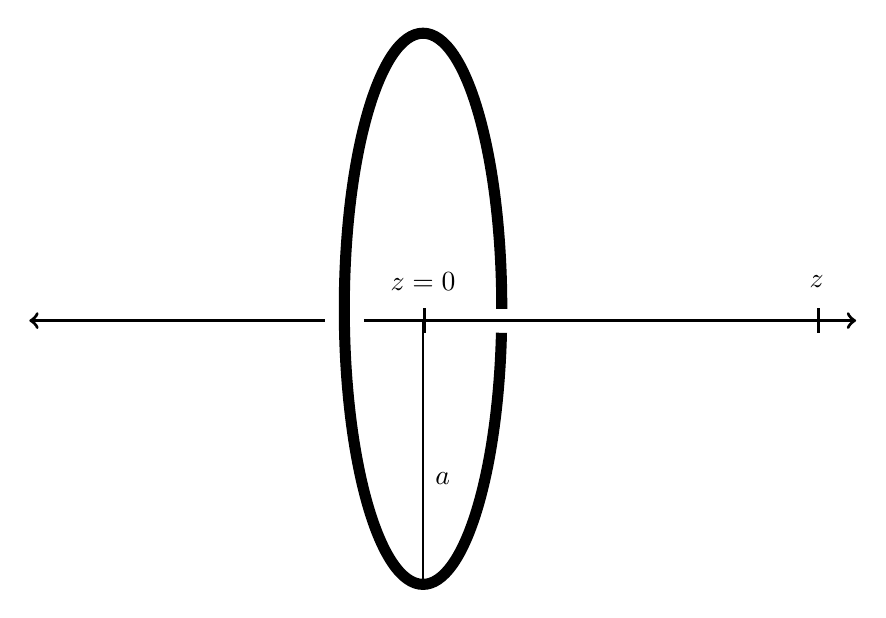
\begin{tikzpicture}
\draw[line width=4] (0,0.15) arc (0:355: 1 and 3.5);
\draw[<-,very thick] (-6,0) -- (-2.25,0);
\draw[very thick] (-1.75,0) -- (-1,0);
\draw[|-,very thick] (-1,0) -- (4,0);
\draw[|->,very thick] (4,0) -- (4.5,0);
\draw (-1,0.5) node {$z=0$};
\draw (4,0.5) node {$z$};
\draw[thick] (-1,0) -- (-1,-3.4);
\draw (-0.75,-2) node {$a$};
\end{tikzpicture}
\caption{Ringworld and its Central Axis}
\end{center}
\end{figure}



To find the gravitational force at a point $z$ on this axis requires adding up all the contributions of bits of the ring. This requires knowing how to integrate, which is a topic covered in a later course, so we will just use the final result of this calculation: the scalar function associated to the gravitational force at a point $z$ on this central axis is given as $$F(z)=\frac{Kz}{(a^2+z^2)^{3/2}},$$ where $K>0$ is a constant, and $a$ is the radius of the ring ($\approx$150 million kilometers). This force points along the axis towards the centre of the ring. (Why?)  Note this result includes the fact $F(0)=0$, which says the net gravitational force at the centre of the ring is 0. 

\begin{enumerate}
\item[(a)] If you are very close to the centre of Ringworld along this central axis, what does the gravitational force look like?  That is, consider the behaviour of the function $F(z)$ for small $z$ -- what simpler function does $F(z)$ look like in this case? 

\item[(b)] If you are very far away from Ringworld along this central axis, what does the gravitational force look like? This is, consider the behaviour of the function $F(z)$ for large $z$ -- what simpler function does F(z) look like in this case?  Comment on the reasonableness of using this simpler function to study the gravitational field at large distances from Ringworld.

\item[(c)] Even though you don't have an expression for the function describing the gravitational force at a general point in space around Ringworld, what do you expect this function to look like when you consider points at large distances from Ringworld in any direction?  What is the reason for your expectation?

\end{enumerate}


\color{blue}
\subsubsection*{Answers}
\begin{parts}
    \part In the case that $z$ is a very small number, we can substitute $z$ for $0$ in the denominator because $z$ is negligible. However, we should be careful not to do the same for the numerator as a coefficient of 0 for the term $K$ will yield $F(z) = 0$ which tells us nothing about the behaviour of $F(z)$. Performing this substitution, we find that as $z \rightarrow 0$, $F(z)$ resembles:
    \begin{equation}
    F(z) = \frac{Kz}{a^3}
    \end{equation}
    \part In approximating the behaviour of $F(z)$ as $z$ becomes very large, we are able to substitute all additive constants with $0$ due to their finite (and therefore negligible) nature relative to $z$ as $z \rightarrow \infty$. In doing so, we get the equation:
    \begin{equation}
    F(z) = \frac{K}{z^2}
    \end{equation}
    
    \part At any point whose distance from the Ringworld is of sufficiently great magnitude, the equation for the force of gravity exerted by the Ringworld upon the object in question could be reasonably approximated by the function we found in 4.b for the force of gravity along the central axis at large values of $z$ ($F(z) = \frac{K}{z^2}$). This is because, as the distance between an object and the Ringworld becomes very large, the constants representing the dimensions of the Ringworld ($a$) become negligible in comparison. If the dimensions of the Ringworld become negligible, it follows that the toroid shape of the Ringworld will have no significant impact on calculations of its force of gravity and therefore that, within a Newtonian framework of physics, the Ringworld is functionally identical to a single point of equivalent mass in three-dimensional space. This means that the the force of gravity exerted by the Ringworld on a small object as a function of $z$ will be the same regardless of the angle at which the object is offset from the Ringworld. Therefore, our previous function as described in 4.b which works with large values of $z$ along the central axis should, in reality, work with large values of $z$ along all axes.
\end{parts}
\color{black}

\end{questions}



\end{document}